\documentclass[10pt]{beamer}
\usepackage{appendix}
\usepackage{mathtools}
\usepackage{floatrow}
\usepackage{amsmath}
\usepackage{cases}
\usepackage{IEEEtrantools}
\usepackage{graphicx}
\usepackage{amsmath}
\usepackage[font=small,labelfont=bf]{subcaption}
\usepackage{amsfonts}
\usepackage{amssymb}
\usepackage{afterpage}
\definecolor{dGreen}{rgb}{0.0, 0.5, 0.0}


% ------ % Set Beamer Style
\useoutertheme{shadow}
\setbeamercolor{background canvas}{bg=white}
\setbeamercolor{title}{bg=dGreen!10,fg=black}
\setbeamercolor{frametitle}{fg=black,bg=dGreen!10}
%\setbeamercolor{subitem}{fg=dGreen} %make subitem or item colored differently
\setbeamersize{text margin left=5mm,text margin right=5mm} 
\usepackage{hyperref}
\hypersetup{
	pdftex,
	%pdftitle={My Project}, % project title
	pdfauthor={Nurlan Jahangirli and friends},     % author
	colorlinks=true,       % false: boxed links; true: colored links
	linkcolor=red,          % color of internal links
	citecolor=brown,        % color of links to bibliography
	urlcolor=blue           % color of external links
}
\floatsetup[table]{capposition=top}
\floatsetup[figure]{capposition=top}
\usepackage{xcolor}
\usepackage[width=1\textwidth,font={small, sf,it},labelfont={color=dGreen,bf, sf},
labelsep=colon, format=plain]{caption}

% ------ % Navigation bar (adding page numbers)
\setbeamertemplate{navigation symbols}{
\ifnum\insertframenumber>\insertmainframenumber%
\relax
\else%
\color{black}{\textbf{\footnotesize \insertframenumber/\insertmainframenumber}}%
\fi%
}
\setbeamertemplate{footline} % remove footline (project name, etc)

% ------ % Set citation style
\usepackage{apacite}
\usepackage{natbib}
\makeatletter
\DeclareRobustCommand\citep
{\begingroup\small\NAT@swatrue\let\NAT@ctype\z@\NAT@partrue
	\@ifstar{\NAT@fulltrue\NAT@citetp}{\NAT@fullfalse\NAT@citetp}}
\makeatother

% ------ % Setting the graphicspath
\graphicspath{{../../}} 

% ------ % Project title and authors
\title{A project}
\subtitle{to do X, Y, Z}
\urldef{\njahangirliWeb}\url{http://development-review.org/}	\urldef{\njahangirliEmail}\url{nurlan.jahangirli@monash.edu}
\newtheorem{proposition}{Proposition}
\author{Nurlan Jahangirli\thanks{Monash U \njahangirliEmail} \\\and friends}
\date{\today}






\begin{document}

\begin{frame}
\maketitle
\end{frame}


\begin{frame}{Intro}

\begin{itemize} 
	\item  \citet{rajan1998financial} claim X. Why?
	\begin{itemize}
		\item[*]  Hello again
	\end{itemize}
	\item 
	\item 
\end{itemize}

\end{frame}





\begin{frame}[label=main]{A Frame with 1 Figure}


\begin{figure}[H]
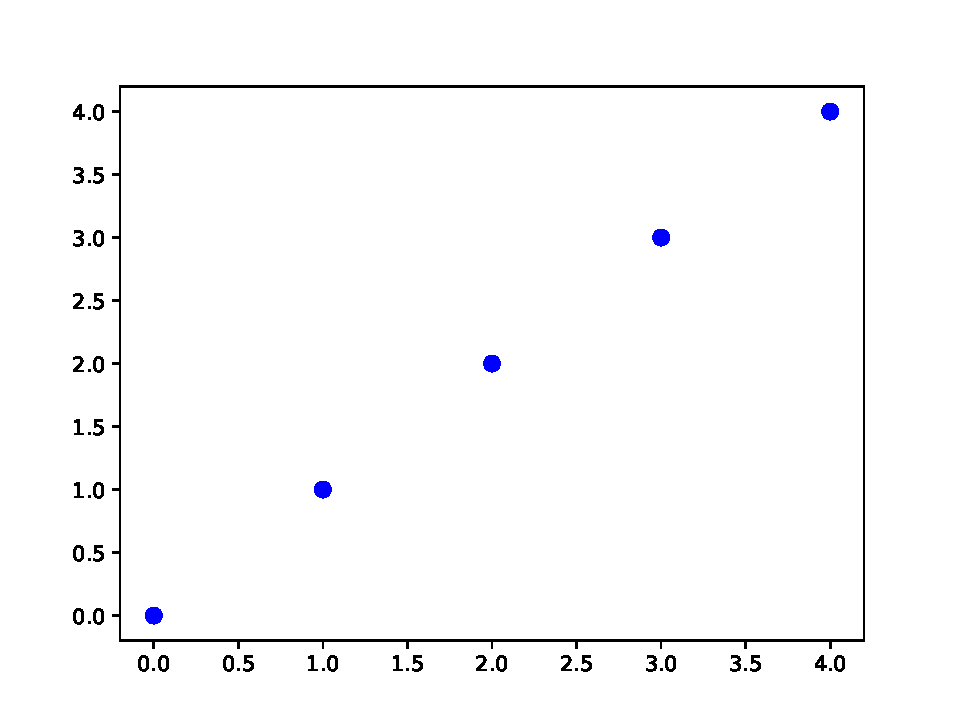
\includegraphics[width=0.7\textwidth]{figures/chart.pdf}
\caption{Example figure. \label{fig:example}}
\end{figure}	
\hyperlink{supplemental}{\beamerbutton{Supplemental checks on X, Y, Z}}

\end{frame}


\begin{frame}{A frame with 3 adjacent figures}
\begin{figure}[H]
\caption{Example-3}
\resizebox{0.97\linewidth}{!}{ 	\centering
\subfloat[][\color{dGreen}Z]{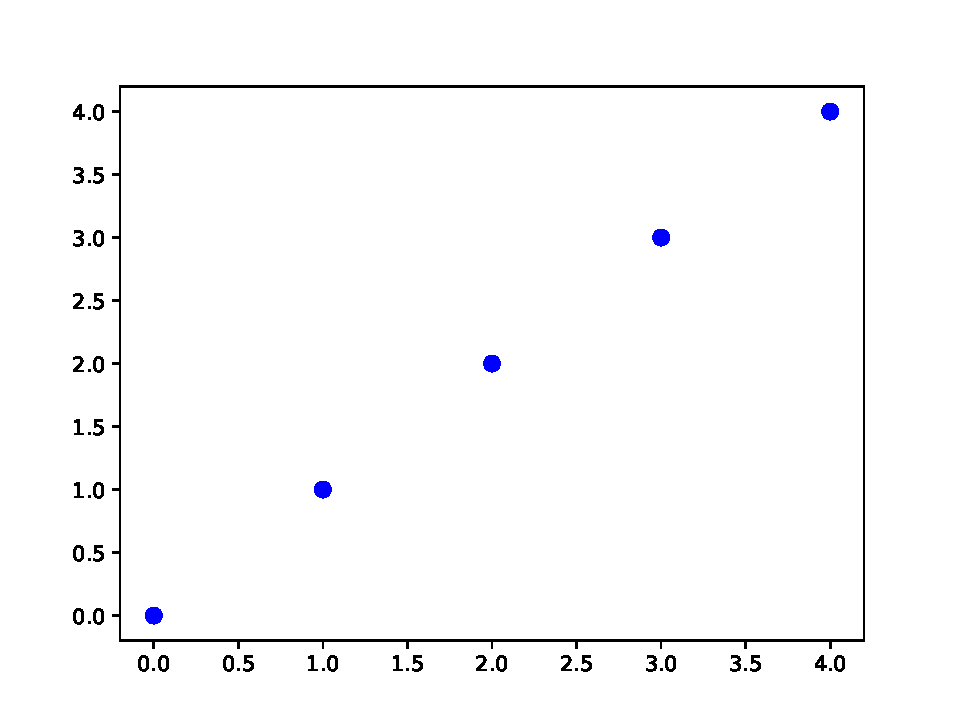
\includegraphics[width=.333\textwidth]{figures/chart.pdf}}
\subfloat[][\color{dGreen}Y]{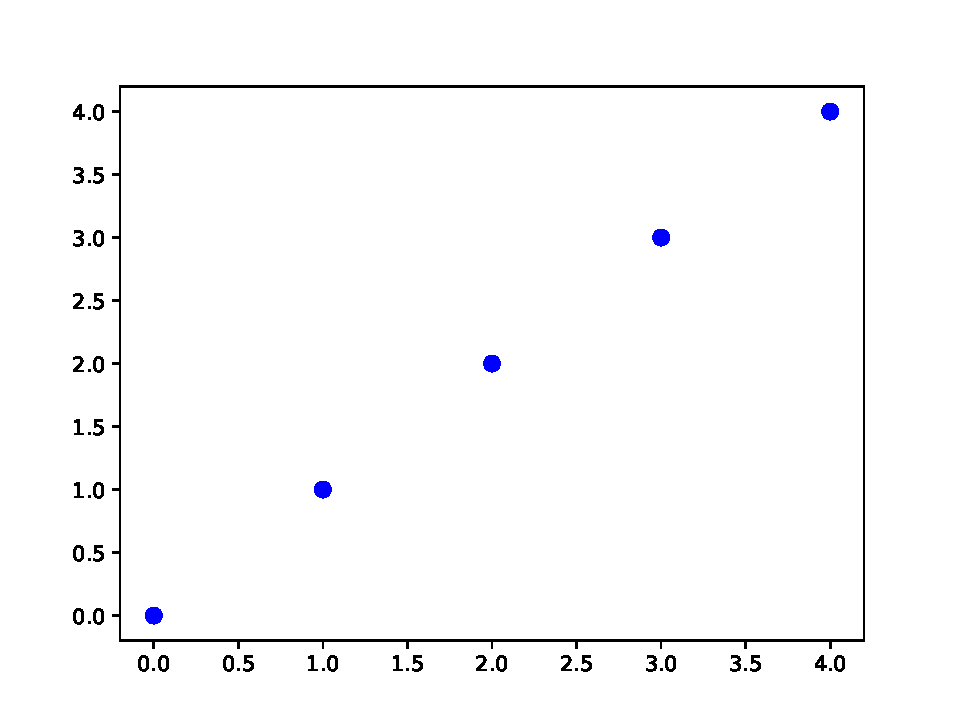
\includegraphics[width=.333\textwidth]{figures/chart.pdf}}
\subfloat[][\color{dGreen}X]{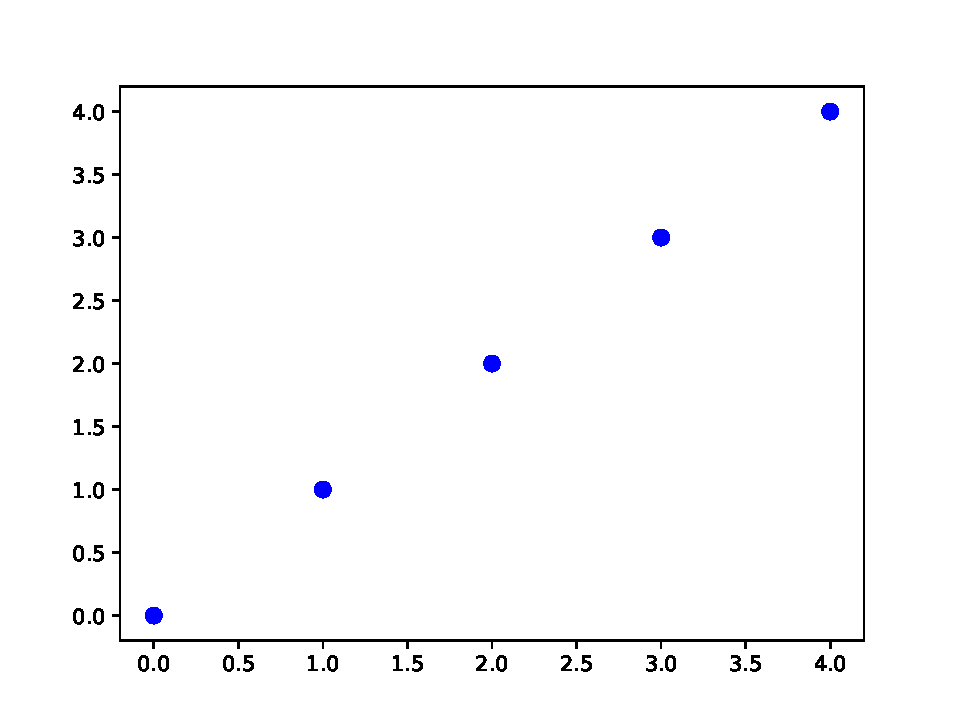
\includegraphics[width=.333\textwidth]{figures/chart.pdf}}
}
\end{figure}

\end{frame}






%%%%%%% APPENDIX

\appendix
\begin{frame}<beamer:0>
\bibliographystyle{chicago}
\bibliography{../../ProjectA.bib} % it is in outputs folder
\end{frame}




\begin{frame}[label=supplemental]{Additional figure}

Back to \hyperlink{main}{\beamerbutton{main}}
\end{frame}

\end{document}